\documentclass[dvips, 10pt]{article}
\usepackage{graphicx}
\usepackage{rotating}
\setlength{\oddsidemargin}{-0.45in}
\setlength{\evensidemargin}{-0.45in}
\setlength{\textwidth}{7.0in}
\setlength{\topmargin}{-0.70in}
\setlength{\textheight}{9.5in}
\pagestyle{myheadings}
\markright{ {\rm {
GLND DSMB Report CLOSED SESSION
 \hspace{2em}
Wed Apr 13 11:52:01 EDT 2011
\hfill
\hspace{3em}
}}}
\headsep=0.2in
\begin{document}
\vspace*{1in}
\begin{center}
{\Huge{CONFIDENTIAL}}
\end{center}
\vspace*{0.5in}
\begin{center}
{\Huge{Efficacy and Mechanisms of GLN Dipeptide in the SICU GLND Trial}}
\end{center}
\vspace*{0.5in}
\begin{center}
{\Huge{Data Safety Monitoring Board Report}}
\end{center}
\vspace*{0.25in}
\begin{center}
{\Huge{
Baseline and Follow-up CLOSED SESSION
}}
\end{center}
\vspace*{1in}
\begin{center}
{\Huge{GLND DSMB Meeting}}
\end{center}
\begin{center}
{\Huge{
May 3, 2011
}}
\end{center}
\begin{center}
{\Huge{10am-2pm EDT}}
\end{center}
\vspace*{1in}
\begin{center}
\noindent
{\Large{Includes patients enrolled and follow-up data received as of April 4, 2011}}
\end{center}
\vspace*{0.5in}
\begin{center}
{\Large{Report prepared  Wed Apr 13 11:52:01 EDT 2011 }}
\end{center}
\clearpage
\vspace*{1in}
\begin{center}
{\Huge{Table of Contents}}
\end{center}
\listoftables
\listoffigures
\clearpage
\begin{table}[tbp]
\caption
{ Patient Characteristics. Tabulation by Treatment. }
\begin{center}
\begin{tabular}{ @{}l@{}
@{}c@{}@{}p{1.5em}@{}@{}c@{}@{}p{1.5em}@{}@{}c@{}
}
\hline

& \parbox{6em}{\begin{center}A\end{center}} && \parbox{6em}{\begin{center}B\end{center}} && \parbox{6em}{\begin{center}Total\end{center}} \\
 & n=69 && n=72 && n=141 \\
 \cline{2-2} \cline{4-4} \cline{6-6} 
 Characteristic &
 \makebox[1.5em]{n}\makebox[3.5em][r]{(\%)} &&
\makebox[1.5em]{n}\makebox[3.5em][r]{(\%)} &&
\makebox[1.5em]{n}\makebox[3.5em][r]{(\%)} \\
 \hline
\\
\parbox[b]{ 70mm }{\raggedright{{\bf Gender }}} &
  &&
  &&
  \\
 \hspace{1em} Male &
 \makebox[1.5em][r]{33}\makebox[3.5em][r]{(47.8)} &&
 \makebox[1.5em][r]{43}\makebox[3.5em][r]{(59.7)} &&
 \makebox[1.5em][r]{76}\makebox[3.5em][r]{(53.9)} \\
 \hspace{1em} Female &
 \makebox[1.5em][r]{36}\makebox[3.5em][r]{(52.2)} &&
 \makebox[1.5em][r]{29}\makebox[3.5em][r]{(40.3)} &&
 \makebox[1.5em][r]{65}\makebox[3.5em][r]{(46.1)} \\
 \vspace{0em} \\
\parbox[b]{ 70mm }{\raggedright{{\bf Race }}} &
  &&
  &&
  \\
 \hspace{1em} Black or African American &
 \makebox[1.5em][r]{14}\makebox[3.5em][r]{(20.3)} &&
 \makebox[1.5em][r]{4}\makebox[3.5em][r]{(5.6)} &&
 \makebox[1.5em][r]{18}\makebox[3.5em][r]{(12.8)} \\
 \hspace{1em} White &
 \makebox[1.5em][r]{55}\makebox[3.5em][r]{(79.7)} &&
 \makebox[1.5em][r]{68}\makebox[3.5em][r]{(94.4)} &&
 \makebox[1.5em][r]{123}\makebox[3.5em][r]{(87.2)} \\
 \vspace{0em} \\
\parbox[b]{ 70mm }{\raggedright{{\bf Hispanic }}} &
  &&
  &&
  \\
 \hspace{1em} No &
 \makebox[1.5em][r]{67}\makebox[3.5em][r]{(97.1)} &&
 \makebox[1.5em][r]{70}\makebox[3.5em][r]{(97.2)} &&
 \makebox[1.5em][r]{137}\makebox[3.5em][r]{(97.2)} \\
 \hspace{1em} Yes &
 \makebox[1.5em][r]{2}\makebox[3.5em][r]{(2.9)} &&
 \makebox[1.5em][r]{2}\makebox[3.5em][r]{(2.8)} &&
 \makebox[1.5em][r]{4}\makebox[3.5em][r]{(2.8)} \\
 \vspace{0em} \\
\parbox[b]{ 70mm }{\raggedright{{\bf Clinical Center }}} &
  &&
  &&
  \\
 \hspace{1em} Colorado &
 \makebox[1.5em][r]{16}\makebox[3.5em][r]{(23.2)} &&
 \makebox[1.5em][r]{17}\makebox[3.5em][r]{(23.6)} &&
 \makebox[1.5em][r]{33}\makebox[3.5em][r]{(23.4)} \\
 \hspace{1em} Emory &
 \makebox[1.5em][r]{27}\makebox[3.5em][r]{(39.1)} &&
 \makebox[1.5em][r]{28}\makebox[3.5em][r]{(38.9)} &&
 \makebox[1.5em][r]{55}\makebox[3.5em][r]{(39.0)} \\
 \hspace{1em} Miriam &
 \makebox[1.5em][r]{4}\makebox[3.5em][r]{(5.8)} &&
 \makebox[1.5em][r]{5}\makebox[3.5em][r]{(6.9)} &&
 \makebox[1.5em][r]{9}\makebox[3.5em][r]{(6.4)} \\
 \hspace{1em} Vanderbilt &
 \makebox[1.5em][r]{20}\makebox[3.5em][r]{(29.0)} &&
 \makebox[1.5em][r]{19}\makebox[3.5em][r]{(26.4)} &&
 \makebox[1.5em][r]{39}\makebox[3.5em][r]{(27.7)} \\
 \hspace{1em} Wisconsin &
 \makebox[1.5em][r]{2}\makebox[3.5em][r]{(2.9)} &&
 \makebox[1.5em][r]{3}\makebox[3.5em][r]{(4.2)} &&
 \makebox[1.5em][r]{5}\makebox[3.5em][r]{(3.5)} \\
 \vspace{0em} \\
\parbox[b]{ 70mm }{\raggedright{{\bf Apache II Score at study entry }}} &
  &&
  &&
  \\
 \hspace{1em} APACHE $ \le $15 &
 \makebox[1.5em][r]{30}\makebox[3.5em][r]{(43.5)} &&
 \makebox[1.5em][r]{36}\makebox[3.5em][r]{(50.0)} &&
 \makebox[1.5em][r]{66}\makebox[3.5em][r]{(46.8)} \\
 \hspace{1em} APACHE $>$15 &
 \makebox[1.5em][r]{39}\makebox[3.5em][r]{(56.5)} &&
 \makebox[1.5em][r]{36}\makebox[3.5em][r]{(50.0)} &&
 \makebox[1.5em][r]{75}\makebox[3.5em][r]{(53.2)} \\
 \vspace{0em} \\
\parbox[b]{ 70mm }{\raggedright{{\bf APACHE II at study entry }}} &
  &&
  &&
  \\
 \hspace{1em} Mean $\pm$ sd &
 $ 16.2 \pm 5.7 $ &&
 $ 15.7 \pm 7.4 $ &&
 $ 16.0 \pm 6.6 $ \\
 \hspace{1em} Median $\pm$ mad &
 $ 16.0 \pm 5.9 $ &&
 $ 15.5 \pm 8.2 $ &&
 $ 16.0 \pm 5.9 $ \\
 \hspace{1em} Range &
 $ 4.0 $ --- $ 29.0 $ &&
 $ 2.0 $ --- $ 36.0 $ &&
 $ 2.0 $ --- $ 36.0 $ \\
 \vspace{0em} \\
\parbox[b]{ 70mm }{\raggedright{{\bf ARDS Present? }}} &
  &&
  &&
  \\
 \hspace{1em} No &
 \makebox[1.5em][r]{58}\makebox[3.5em][r]{(84.1)} &&
 \makebox[1.5em][r]{66}\makebox[3.5em][r]{(91.7)} &&
 \makebox[1.5em][r]{124}\makebox[3.5em][r]{(87.9)} \\
 \hspace{1em} Yes &
 \makebox[1.5em][r]{11}\makebox[3.5em][r]{(15.9)} &&
 \makebox[1.5em][r]{6}\makebox[3.5em][r]{(8.3)} &&
 \makebox[1.5em][r]{17}\makebox[3.5em][r]{(12.1)} \\
 \vspace{0em} \\
\parbox[b]{ 70mm }{\raggedright{{\bf On Ventilator at Entry }}} &
  &&
  &&
  \\
 \hspace{1em} No &
 \makebox[1.5em][r]{19}\makebox[3.5em][r]{(27.5)} &&
 \makebox[1.5em][r]{30}\makebox[3.5em][r]{(41.7)} &&
 \makebox[1.5em][r]{49}\makebox[3.5em][r]{(34.8)} \\
 \hspace{1em} Yes &
 \makebox[1.5em][r]{50}\makebox[3.5em][r]{(72.5)} &&
 \makebox[1.5em][r]{42}\makebox[3.5em][r]{(58.3)} &&
 \makebox[1.5em][r]{92}\makebox[3.5em][r]{(65.2)} \\
 \vspace{0em} \\
\parbox[b]{ 70mm }{\raggedright{{\bf Age at Consent }}} &
  &&
 n=71 &&
 n=140 \\
 \hspace{1em} Mean $\pm$ sd &
 $ 60.2 \pm 14.0 $ &&
 $ 60.6 \pm 13.3 $ &&
 $ 60.4 \pm 13.6 $ \\
 \hspace{1em} Median $\pm$ mad &
 $ 61.7 \pm 12.1 $ &&
 $ 61.3 \pm 10.9 $ &&
 $ 61.3 \pm 11.8 $ \\
 \hspace{1em} Range &
 $ 22.4 $ --- $ 83.1 $ &&
 $ 22.8 $ --- $ 86.4 $ &&
 $ 22.4 $ --- $ 86.4 $ \\
 \vspace{0em} \\
\hline \\ 
\end{tabular}

\parbox{ 5in }{ mad - median of the absolute values of the deviation from the median } \\
 \vspace{1em}\end{center}
 \end{table}
\clearpage
\begin{table}[tbp]
\caption
{ Patient Characteristics (Continued). Tabulation by Treatment. }
\begin{center}
\begin{tabular}{ @{}l@{}
@{}c@{}@{}p{1.5em}@{}@{}c@{}@{}p{1.5em}@{}@{}c@{}
}
\hline

& \parbox{6em}{\begin{center}A\end{center}} && \parbox{6em}{\begin{center}B\end{center}} && \parbox{6em}{\begin{center}Total\end{center}} \\
 & n=69 && n=72 && n=141 \\
 \cline{2-2} \cline{4-4} \cline{6-6} 
 Characteristic &
 \makebox[1.5em]{n}\makebox[3.5em][r]{(\%)} &&
\makebox[1.5em]{n}\makebox[3.5em][r]{(\%)} &&
\makebox[1.5em]{n}\makebox[3.5em][r]{(\%)} \\
 \hline
\\
\parbox[b]{ 70mm }{\raggedright{{\bf BMI (kg/m*m) }}} &
  &&
  &&
  \\
 \hspace{1em} Mean $\pm$ sd &
 $ 27.0 \pm 6.0 $ &&
 $ 26.6 \pm 6.3 $ &&
 $ 26.8 \pm 6.1 $ \\
 \hspace{1em} Median $\pm$ mad &
 $ 26.9 \pm 6.7 $ &&
 $ 26.8 \pm 7.5 $ &&
 $ 26.9 \pm 7.0 $ \\
 \hspace{1em} Range &
 $ 13.6 $ --- $ 39.7 $ &&
 $ 12.5 $ --- $ 39.2 $ &&
 $ 12.5 $ --- $ 39.7 $ \\
 \vspace{0em} \\
\parbox[b]{ 70mm }{\raggedright{{\bf Index Surgery }}} &
  &&
  &&
  \\
 \hspace{1em} CABG &
 \makebox[1.5em][r]{3}\makebox[3.5em][r]{(4.3)} &&
 \makebox[1.5em][r]{2}\makebox[3.5em][r]{(2.8)} &&
 \makebox[1.5em][r]{5}\makebox[3.5em][r]{(3.5)} \\
 \hspace{1em} Cardiac valve &
 \makebox[1.5em][r]{3}\makebox[3.5em][r]{(4.3)} &&
 \makebox[1.5em][r]{2}\makebox[3.5em][r]{(2.8)} &&
 \makebox[1.5em][r]{5}\makebox[3.5em][r]{(3.5)} \\
 \hspace{1em} Intestinal resection &
 \makebox[1.5em][r]{44}\makebox[3.5em][r]{(63.8)} &&
 \makebox[1.5em][r]{51}\makebox[3.5em][r]{(70.8)} &&
 \makebox[1.5em][r]{95}\makebox[3.5em][r]{(67.4)} \\
 \hspace{1em} Peritontis &
 \makebox[1.5em][r]{1}\makebox[3.5em][r]{(1.4)} &&
 \makebox[1.5em][r]{1}\makebox[3.5em][r]{(1.4)} &&
 \makebox[1.5em][r]{2}\makebox[3.5em][r]{(1.4)} \\
 \hspace{1em} Upper GI resection &
 \makebox[1.5em][r]{1}\makebox[3.5em][r]{(1.4)} &&
 \makebox[1.5em][r]{3}\makebox[3.5em][r]{(4.2)} &&
 \makebox[1.5em][r]{4}\makebox[3.5em][r]{(2.8)} \\
 \hspace{1em} Vascular &
 \makebox[1.5em][r]{17}\makebox[3.5em][r]{(24.6)} &&
 \makebox[1.5em][r]{13}\makebox[3.5em][r]{(18.1)} &&
 \makebox[1.5em][r]{30}\makebox[3.5em][r]{(21.3)} \\
 \vspace{0em} \\
\parbox[b]{ 70mm }{\raggedright{{\bf Primary Diagnosis leading to Elig. Surgery }}} &
  &&
  &&
  \\
 \hspace{1em} Acute mesenteric ischemia &
 \makebox[1.5em][r]{0}\makebox[3.5em][r]{(0.0)} &&
 \makebox[1.5em][r]{1}\makebox[3.5em][r]{(1.4)} &&
 \makebox[1.5em][r]{1}\makebox[3.5em][r]{(0.7)} \\
 \hspace{1em} Acute post-MI ventricular septal defect &
 \makebox[1.5em][r]{0}\makebox[3.5em][r]{(0.0)} &&
 \makebox[1.5em][r]{1}\makebox[3.5em][r]{(1.4)} &&
 \makebox[1.5em][r]{1}\makebox[3.5em][r]{(0.7)} \\
 \hspace{1em} Aortic dissection &
 \makebox[1.5em][r]{1}\makebox[3.5em][r]{(1.4)} &&
 \makebox[1.5em][r]{0}\makebox[3.5em][r]{(0.0)} &&
 \makebox[1.5em][r]{1}\makebox[3.5em][r]{(0.7)} \\
 \hspace{1em} Benign intestinal tumors &
 \makebox[1.5em][r]{1}\makebox[3.5em][r]{(1.4)} &&
 \makebox[1.5em][r]{0}\makebox[3.5em][r]{(0.0)} &&
 \makebox[1.5em][r]{1}\makebox[3.5em][r]{(0.7)} \\
 \hspace{1em} CAD &
 \makebox[1.5em][r]{3}\makebox[3.5em][r]{(4.3)} &&
 \makebox[1.5em][r]{2}\makebox[3.5em][r]{(2.8)} &&
 \makebox[1.5em][r]{5}\makebox[3.5em][r]{(3.5)} \\
 \hspace{1em} Chronic inflammation of abdominal wound &
 \makebox[1.5em][r]{1}\makebox[3.5em][r]{(1.4)} &&
 \makebox[1.5em][r]{0}\makebox[3.5em][r]{(0.0)} &&
 \makebox[1.5em][r]{1}\makebox[3.5em][r]{(0.7)} \\
 \hspace{1em} Colonic necrosis &
 \makebox[1.5em][r]{0}\makebox[3.5em][r]{(0.0)} &&
 \makebox[1.5em][r]{1}\makebox[3.5em][r]{(1.4)} &&
 \makebox[1.5em][r]{1}\makebox[3.5em][r]{(0.7)} \\
 \hspace{1em} Colostomy takedown &
 \makebox[1.5em][r]{1}\makebox[3.5em][r]{(1.4)} &&
 \makebox[1.5em][r]{1}\makebox[3.5em][r]{(1.4)} &&
 \makebox[1.5em][r]{2}\makebox[3.5em][r]{(1.4)} \\
 \hspace{1em} Diffuse gastric polyposis &
 \makebox[1.5em][r]{0}\makebox[3.5em][r]{(0.0)} &&
 \makebox[1.5em][r]{1}\makebox[3.5em][r]{(1.4)} &&
 \makebox[1.5em][r]{1}\makebox[3.5em][r]{(0.7)} \\
 \hspace{1em} Diverticulitis &
 \makebox[1.5em][r]{0}\makebox[3.5em][r]{(0.0)} &&
 \makebox[1.5em][r]{1}\makebox[3.5em][r]{(1.4)} &&
 \makebox[1.5em][r]{1}\makebox[3.5em][r]{(0.7)} \\
 \hspace{1em} Gastric emptying problems(Hx of GSW to a &
 \makebox[1.5em][r]{0}\makebox[3.5em][r]{(0.0)} &&
 \makebox[1.5em][r]{1}\makebox[3.5em][r]{(1.4)} &&
 \makebox[1.5em][r]{1}\makebox[3.5em][r]{(0.7)} \\
 \hspace{1em} Gastric volvulus secondary to paraesopha &
 \makebox[1.5em][r]{0}\makebox[3.5em][r]{(0.0)} &&
 \makebox[1.5em][r]{1}\makebox[3.5em][r]{(1.4)} &&
 \makebox[1.5em][r]{1}\makebox[3.5em][r]{(0.7)} \\
 \hspace{1em} Inflammatory bowel disease &
 \makebox[1.5em][r]{1}\makebox[3.5em][r]{(1.4)} &&
 \makebox[1.5em][r]{3}\makebox[3.5em][r]{(4.2)} &&
 \makebox[1.5em][r]{4}\makebox[3.5em][r]{(2.8)} \\
 \hspace{1em} Intestinal anatamosis leak -$>$ peritoniti &
 \makebox[1.5em][r]{1}\makebox[3.5em][r]{(1.4)} &&
 \makebox[1.5em][r]{0}\makebox[3.5em][r]{(0.0)} &&
 \makebox[1.5em][r]{1}\makebox[3.5em][r]{(0.7)} \\
 \hspace{1em} Intestinal fistula/stricture/adh &
 \makebox[1.5em][r]{12}\makebox[3.5em][r]{(17.4)} &&
 \makebox[1.5em][r]{17}\makebox[3.5em][r]{(23.6)} &&
 \makebox[1.5em][r]{29}\makebox[3.5em][r]{(20.6)} \\
 \hspace{1em} Intestinal ischemia &
 \makebox[1.5em][r]{4}\makebox[3.5em][r]{(5.8)} &&
 \makebox[1.5em][r]{12}\makebox[3.5em][r]{(16.7)} &&
 \makebox[1.5em][r]{16}\makebox[3.5em][r]{(11.3)} \\
 \hspace{1em} Intestinal obstruction &
 \makebox[1.5em][r]{10}\makebox[3.5em][r]{(14.5)} &&
 \makebox[1.5em][r]{8}\makebox[3.5em][r]{(11.1)} &&
 \makebox[1.5em][r]{18}\makebox[3.5em][r]{(12.8)} \\
 \hspace{1em} Intestinal perforation &
 \makebox[1.5em][r]{6}\makebox[3.5em][r]{(8.7)} &&
 \makebox[1.5em][r]{8}\makebox[3.5em][r]{(11.1)} &&
 \makebox[1.5em][r]{14}\makebox[3.5em][r]{(9.9)} \\
 \hspace{1em} Intestinal pseudo obstruction &
 \makebox[1.5em][r]{1}\makebox[3.5em][r]{(1.4)} &&
 \makebox[1.5em][r]{0}\makebox[3.5em][r]{(0.0)} &&
 \makebox[1.5em][r]{1}\makebox[3.5em][r]{(0.7)} \\
 \hspace{1em} Intraabdominal abscess \& anastomotic bre &
 \makebox[1.5em][r]{0}\makebox[3.5em][r]{(0.0)} &&
 \makebox[1.5em][r]{1}\makebox[3.5em][r]{(1.4)} &&
 \makebox[1.5em][r]{1}\makebox[3.5em][r]{(0.7)} \\
 \hspace{1em} Intractable cervical esophageal strictur &
 \makebox[1.5em][r]{1}\makebox[3.5em][r]{(1.4)} &&
 \makebox[1.5em][r]{0}\makebox[3.5em][r]{(0.0)} &&
 \makebox[1.5em][r]{1}\makebox[3.5em][r]{(0.7)} \\
 \hspace{1em} Mesenteric ischemia, jejunal gangrene &
 \makebox[1.5em][r]{1}\makebox[3.5em][r]{(1.4)} &&
 \makebox[1.5em][r]{0}\makebox[3.5em][r]{(0.0)} &&
 \makebox[1.5em][r]{1}\makebox[3.5em][r]{(0.7)} \\
 \hspace{1em} Occulusion of aorta &
 \makebox[1.5em][r]{1}\makebox[3.5em][r]{(1.4)} &&
 \makebox[1.5em][r]{0}\makebox[3.5em][r]{(0.0)} &&
 \makebox[1.5em][r]{1}\makebox[3.5em][r]{(0.7)} \\
 \hspace{1em} Paraesophageal hernia after gastric bypa &
 \makebox[1.5em][r]{1}\makebox[3.5em][r]{(1.4)} &&
 \makebox[1.5em][r]{0}\makebox[3.5em][r]{(0.0)} &&
 \makebox[1.5em][r]{1}\makebox[3.5em][r]{(0.7)} \\
 \hspace{1em} Peritonitis &
 \makebox[1.5em][r]{0}\makebox[3.5em][r]{(0.0)} &&
 \makebox[1.5em][r]{1}\makebox[3.5em][r]{(1.4)} &&
 \makebox[1.5em][r]{1}\makebox[3.5em][r]{(0.7)} \\
 \hspace{1em} Pneumatosis intestinalis &
 \makebox[1.5em][r]{0}\makebox[3.5em][r]{(0.0)} &&
 \makebox[1.5em][r]{1}\makebox[3.5em][r]{(1.4)} &&
 \makebox[1.5em][r]{1}\makebox[3.5em][r]{(0.7)} \\
 \hspace{1em} Rectal  prolapse and fecal incontinence &
 \makebox[1.5em][r]{1}\makebox[3.5em][r]{(1.4)} &&
 \makebox[1.5em][r]{0}\makebox[3.5em][r]{(0.0)} &&
 \makebox[1.5em][r]{1}\makebox[3.5em][r]{(0.7)} \\
 \hspace{1em} Recurrent gastroesophageal reflux dis. &
 \makebox[1.5em][r]{1}\makebox[3.5em][r]{(1.4)} &&
 \makebox[1.5em][r]{0}\makebox[3.5em][r]{(0.0)} &&
 \makebox[1.5em][r]{1}\makebox[3.5em][r]{(0.7)} \\
 \hspace{1em} Toxic colitis &
 \makebox[1.5em][r]{2}\makebox[3.5em][r]{(2.9)} &&
 \makebox[1.5em][r]{1}\makebox[3.5em][r]{(1.4)} &&
 \makebox[1.5em][r]{3}\makebox[3.5em][r]{(2.1)} \\
 \hspace{1em} Valve malfunction &
 \makebox[1.5em][r]{3}\makebox[3.5em][r]{(4.3)} &&
 \makebox[1.5em][r]{2}\makebox[3.5em][r]{(2.8)} &&
 \makebox[1.5em][r]{5}\makebox[3.5em][r]{(3.5)} \\
 \hspace{1em} Vascular aneurysm &
 \makebox[1.5em][r]{12}\makebox[3.5em][r]{(17.4)} &&
 \makebox[1.5em][r]{8}\makebox[3.5em][r]{(11.1)} &&
 \makebox[1.5em][r]{20}\makebox[3.5em][r]{(14.2)} \\
 \hspace{1em} Vascular stenosis &
 \makebox[1.5em][r]{2}\makebox[3.5em][r]{(2.9)} &&
 \makebox[1.5em][r]{0}\makebox[3.5em][r]{(0.0)} &&
 \makebox[1.5em][r]{2}\makebox[3.5em][r]{(1.4)} \\
 \hspace{1em} Vascular thrombosis &
 \makebox[1.5em][r]{1}\makebox[3.5em][r]{(1.4)} &&
 \makebox[1.5em][r]{0}\makebox[3.5em][r]{(0.0)} &&
 \makebox[1.5em][r]{1}\makebox[3.5em][r]{(0.7)} \\
 \hspace{1em} Ventral hernia repair; poss. peritonitis &
 \makebox[1.5em][r]{1}\makebox[3.5em][r]{(1.4)} &&
 \makebox[1.5em][r]{0}\makebox[3.5em][r]{(0.0)} &&
 \makebox[1.5em][r]{1}\makebox[3.5em][r]{(0.7)} \\
 \vspace{0em} \\
\hline \\ 
\end{tabular}
\end{center}
 \end{table}
\clearpage
\begin{table}[tbp]
\caption
{ Patient Characteristics (Continued). Tabulation by Treatment. }
\begin{center}
\begin{tabular}{ @{}l@{}
@{}c@{}@{}p{1.5em}@{}@{}c@{}@{}p{1.5em}@{}@{}c@{}
}
\hline

& \parbox{6em}{\begin{center}A\end{center}} && \parbox{6em}{\begin{center}B\end{center}} && \parbox{6em}{\begin{center}Total\end{center}} \\
 & n=69 && n=72 && n=141 \\
 \cline{2-2} \cline{4-4} \cline{6-6} 
 Characteristic &
 \makebox[1.5em]{n}\makebox[3.5em][r]{(\%)} &&
\makebox[1.5em]{n}\makebox[3.5em][r]{(\%)} &&
\makebox[1.5em]{n}\makebox[3.5em][r]{(\%)} \\
 \hline
\\
\parbox[b]{ 70mm }{\raggedright{{\bf Days from Index Surgery to Enrollment }}} &
  &&
  &&
  \\
 \hspace{1em} Mean $\pm$ sd &
 $ 4.5 \pm 2.8 $ &&
 $ 4.4 \pm 2.9 $ &&
 $ 4.4 \pm 2.9 $ \\
 \hspace{1em} Median $\pm$ mad &
 $ 4.0 \pm 3.0 $ &&
 $ 3.0 \pm 1.5 $ &&
 $ 4.0 \pm 3.0 $ \\
 \hspace{1em} Range &
 $ 0.0 $ --- $ 14.0 $ &&
 $ 1.0 $ --- $ 13.0 $ &&
 $ 0.0 $ --- $ 14.0 $ \\
 \vspace{0em} \\
\parbox[b]{ 70mm }{\raggedright{{\bf Intra-aortic pump? }}} &
  &&
  &&
  \\
 \hspace{1em} No &
 \makebox[1.5em][r]{68}\makebox[3.5em][r]{(98.6)} &&
 \makebox[1.5em][r]{69}\makebox[3.5em][r]{(95.8)} &&
 \makebox[1.5em][r]{137}\makebox[3.5em][r]{(97.2)} \\
 \hspace{1em} Yes &
 \makebox[1.5em][r]{1}\makebox[3.5em][r]{(1.4)} &&
 \makebox[1.5em][r]{3}\makebox[3.5em][r]{(4.2)} &&
 \makebox[1.5em][r]{4}\makebox[3.5em][r]{(2.8)} \\
 \vspace{0em} \\
\parbox[b]{ 70mm }{\raggedright{{\bf Pre-Nosocomial infection? }}} &
  &&
  &&
  \\
 \hspace{1em} No &
 \makebox[1.5em][r]{45}\makebox[3.5em][r]{(65.2)} &&
 \makebox[1.5em][r]{47}\makebox[3.5em][r]{(65.3)} &&
 \makebox[1.5em][r]{92}\makebox[3.5em][r]{(65.2)} \\
 \hspace{1em} Yes &
 \makebox[1.5em][r]{24}\makebox[3.5em][r]{(34.8)} &&
 \makebox[1.5em][r]{25}\makebox[3.5em][r]{(34.7)} &&
 \makebox[1.5em][r]{49}\makebox[3.5em][r]{(34.8)} \\
 \vspace{0em} \\
\parbox[b]{ 70mm }{\raggedright{{\bf Nutritional status }}} &
  &&
  &&
  \\
 \hspace{1em} No malnutrition &
 \makebox[1.5em][r]{31}\makebox[3.5em][r]{(44.9)} &&
 \makebox[1.5em][r]{28}\makebox[3.5em][r]{(38.9)} &&
 \makebox[1.5em][r]{59}\makebox[3.5em][r]{(41.8)} \\
 \hspace{1em} Mild to moderate malnutrition &
 \makebox[1.5em][r]{26}\makebox[3.5em][r]{(37.7)} &&
 \makebox[1.5em][r]{35}\makebox[3.5em][r]{(48.6)} &&
 \makebox[1.5em][r]{61}\makebox[3.5em][r]{(43.3)} \\
 \hspace{1em} Severe malnutrition &
 \makebox[1.5em][r]{12}\makebox[3.5em][r]{(17.4)} &&
 \makebox[1.5em][r]{9}\makebox[3.5em][r]{(12.5)} &&
 \makebox[1.5em][r]{21}\makebox[3.5em][r]{(14.9)} \\
 \vspace{0em} \\
\parbox[b]{ 70mm }{\raggedright{{\bf WBC count (1000/uL) }}} &
  &&
  &&
  \\
 \hspace{1em} Mean $\pm$ sd &
 $ 13.9 \pm 6.6 $ &&
 $ 14.3 \pm 9.0 $ &&
 $ 14.1 \pm 7.9 $ \\
 \hspace{1em} Median $\pm$ mad &
 $ 13.1 \pm 6.7 $ &&
 $ 11.8 \pm 6.8 $ &&
 $ 12.3 \pm 6.4 $ \\
 \hspace{1em} Range &
 $ 1.0 $ --- $ 35.6 $ &&
 $ 3.0 $ --- $ 51.0 $ &&
 $ 1.0 $ --- $ 51.0 $ \\
 \vspace{0em} \\
\hline \\ 
\end{tabular}
\end{center}
 \end{table}
\clearpage
\begin{table}[tbp]
\caption
{ Patient Characteristics (Continued). Tabulation by Treatment. }
\begin{center}
\begin{tabular}{ @{}l@{}
@{}c@{}@{}p{1.5em}@{}@{}c@{}@{}p{1.5em}@{}@{}c@{}
}
\hline

& \parbox{6em}{\begin{center}A\end{center}} && \parbox{6em}{\begin{center}B\end{center}} && \parbox{6em}{\begin{center}Total\end{center}} \\
 & n=69 && n=72 && n=141 \\
 \cline{2-2} \cline{4-4} \cline{6-6} 
 Characteristic &
 \makebox[1.5em]{n}\makebox[3.5em][r]{(\%)} &&
\makebox[1.5em]{n}\makebox[3.5em][r]{(\%)} &&
\makebox[1.5em]{n}\makebox[3.5em][r]{(\%)} \\
 \hline
\\
\parbox[b]{ 70mm }{\raggedright{{\bf PN Indication - Illeus }}} &
  &&
  &&
  \\
 \hspace{1em} No &
 \makebox[1.5em][r]{34}\makebox[3.5em][r]{(49.3)} &&
 \makebox[1.5em][r]{34}\makebox[3.5em][r]{(47.2)} &&
 \makebox[1.5em][r]{68}\makebox[3.5em][r]{(48.2)} \\
 \hspace{1em} Yes &
 \makebox[1.5em][r]{35}\makebox[3.5em][r]{(50.7)} &&
 \makebox[1.5em][r]{38}\makebox[3.5em][r]{(52.8)} &&
 \makebox[1.5em][r]{73}\makebox[3.5em][r]{(51.8)} \\
 \vspace{0em} \\
\parbox[b]{ 70mm }{\raggedright{{\bf PN Indication - Ischemic bowel }}} &
  &&
  &&
  \\
 \hspace{1em} No &
 \makebox[1.5em][r]{60}\makebox[3.5em][r]{(87.0)} &&
 \makebox[1.5em][r]{59}\makebox[3.5em][r]{(81.9)} &&
 \makebox[1.5em][r]{119}\makebox[3.5em][r]{(84.4)} \\
 \hspace{1em} Yes &
 \makebox[1.5em][r]{9}\makebox[3.5em][r]{(13.0)} &&
 \makebox[1.5em][r]{13}\makebox[3.5em][r]{(18.1)} &&
 \makebox[1.5em][r]{22}\makebox[3.5em][r]{(15.6)} \\
 \vspace{0em} \\
\parbox[b]{ 70mm }{\raggedright{{\bf PN Indication - Hemodynamic instab. }}} &
  &&
  &&
  \\
 \hspace{1em} No &
 \makebox[1.5em][r]{56}\makebox[3.5em][r]{(81.2)} &&
 \makebox[1.5em][r]{60}\makebox[3.5em][r]{(83.3)} &&
 \makebox[1.5em][r]{116}\makebox[3.5em][r]{(82.3)} \\
 \hspace{1em} Yes &
 \makebox[1.5em][r]{13}\makebox[3.5em][r]{(18.8)} &&
 \makebox[1.5em][r]{12}\makebox[3.5em][r]{(16.7)} &&
 \makebox[1.5em][r]{25}\makebox[3.5em][r]{(17.7)} \\
 \vspace{0em} \\
\parbox[b]{ 70mm }{\raggedright{{\bf PN Indication - Intolerence to ent. }}} &
  &&
  &&
  \\
 \hspace{1em} No &
 \makebox[1.5em][r]{65}\makebox[3.5em][r]{(94.2)} &&
 \makebox[1.5em][r]{67}\makebox[3.5em][r]{(93.1)} &&
 \makebox[1.5em][r]{132}\makebox[3.5em][r]{(93.6)} \\
 \hspace{1em} Yes &
 \makebox[1.5em][r]{4}\makebox[3.5em][r]{(5.8)} &&
 \makebox[1.5em][r]{5}\makebox[3.5em][r]{(6.9)} &&
 \makebox[1.5em][r]{9}\makebox[3.5em][r]{(6.4)} \\
 \vspace{0em} \\
\parbox[b]{ 70mm }{\raggedright{{\bf PN Indication - Bowel obstruction }}} &
  &&
  &&
  \\
 \hspace{1em} No &
 \makebox[1.5em][r]{65}\makebox[3.5em][r]{(94.2)} &&
 \makebox[1.5em][r]{69}\makebox[3.5em][r]{(95.8)} &&
 \makebox[1.5em][r]{134}\makebox[3.5em][r]{(95.0)} \\
 \hspace{1em} Yes &
 \makebox[1.5em][r]{4}\makebox[3.5em][r]{(5.8)} &&
 \makebox[1.5em][r]{3}\makebox[3.5em][r]{(4.2)} &&
 \makebox[1.5em][r]{7}\makebox[3.5em][r]{(5.0)} \\
 \vspace{0em} \\
\parbox[b]{ 70mm }{\raggedright{{\bf PN Indication - Other }}} &
  &&
  &&
  \\
 \hspace{1em} No &
 \makebox[1.5em][r]{50}\makebox[3.5em][r]{(72.5)} &&
 \makebox[1.5em][r]{47}\makebox[3.5em][r]{(65.3)} &&
 \makebox[1.5em][r]{97}\makebox[3.5em][r]{(68.8)} \\
 \hspace{1em} Yes &
 \makebox[1.5em][r]{19}\makebox[3.5em][r]{(27.5)} &&
 \makebox[1.5em][r]{25}\makebox[3.5em][r]{(34.7)} &&
 \makebox[1.5em][r]{44}\makebox[3.5em][r]{(31.2)} \\
 \vspace{0em} \\
\parbox[b]{ 70mm }{\raggedright{{\bf Enteral nutrition within 30 days prior to entry }}} &
  &&
  &&
  \\
 \hspace{1em} No &
 \makebox[1.5em][r]{56}\makebox[3.5em][r]{(81.2)} &&
 \makebox[1.5em][r]{66}\makebox[3.5em][r]{(91.7)} &&
 \makebox[1.5em][r]{122}\makebox[3.5em][r]{(86.5)} \\
 \hspace{1em} Yes &
 \makebox[1.5em][r]{13}\makebox[3.5em][r]{(18.8)} &&
 \makebox[1.5em][r]{6}\makebox[3.5em][r]{(8.3)} &&
 \makebox[1.5em][r]{19}\makebox[3.5em][r]{(13.5)} \\
 \vspace{0em} \\
\parbox[b]{ 70mm }{\raggedright{{\bf Parenteral nutrition within 30 days prior to entry }}} &
  &&
  &&
  \\
 \hspace{1em} No &
 \makebox[1.5em][r]{16}\makebox[3.5em][r]{(23.2)} &&
 \makebox[1.5em][r]{12}\makebox[3.5em][r]{(16.7)} &&
 \makebox[1.5em][r]{28}\makebox[3.5em][r]{(19.9)} \\
 \hspace{1em} Yes &
 \makebox[1.5em][r]{53}\makebox[3.5em][r]{(76.8)} &&
 \makebox[1.5em][r]{60}\makebox[3.5em][r]{(83.3)} &&
 \makebox[1.5em][r]{113}\makebox[3.5em][r]{(80.1)} \\
 \vspace{0em} \\
\parbox[b]{ 70mm }{\raggedright{{\bf APACHE II first day SICU }}} &
  &&
  &&
  \\
 \hspace{1em} Mean $\pm$ sd &
 $ 23.2 \pm 7.6 $ &&
 $ 22.1 \pm 7.7 $ &&
 $ 22.6 \pm 7.6 $ \\
 \hspace{1em} Median $\pm$ mad &
 $ 24.0 \pm 5.9 $ &&
 $ 22.5 \pm 6.7 $ &&
 $ 23.0 \pm 5.9 $ \\
 \hspace{1em} Range &
 $ 6.0 $ --- $ 40.0 $ &&
 $ 6.0 $ --- $ 43.0 $ &&
 $ 6.0 $ --- $ 43.0 $ \\
 \vspace{0em} \\
\hline \\ 
\end{tabular}
\end{center}
 \end{table}
\begin{table}[tbp]
\caption
{ Duration of Hospitalization. Tabulation by Treatment. }
\begin{center}
\begin{tabular}{ @{}l@{}
@{}c@{}@{}p{1.5em}@{}@{}c@{}@{}p{1.5em}@{}@{}c@{}
}
\hline

& \parbox{6em}{\begin{center}A\end{center}} && \parbox{6em}{\begin{center}B\end{center}} && \parbox{6em}{\begin{center}Total\end{center}} \\
 & n=69 && n=72 && n=141 \\
 \cline{2-2} \cline{4-4} \cline{6-6} 
 Characteristic &
 \makebox[1.5em]{n}\makebox[3.5em][r]{(\%)} &&
\makebox[1.5em]{n}\makebox[3.5em][r]{(\%)} &&
\makebox[1.5em]{n}\makebox[3.5em][r]{(\%)} \\
 \hline
\\
\parbox[b]{ 70mm }{\raggedright{{\bf Total days in the hospital }}} &
 n=67 &&
 n=71 &&
 n=138 \\
 \hspace{1em} Mean $\pm$ sd &
 $ 31.0 \pm 19.6 $ &&
 $ 29.3 \pm 21.2 $ &&
 $ 30.1 \pm 20.4 $ \\
 \hspace{1em} Median $\pm$ mad &
 $ 25.0 \pm 13.3 $ &&
 $ 24.0 \pm 13.3 $ &&
 $ 24.5 \pm 14.1 $ \\
 \hspace{1em} Range &
 $ 7.0 $ --- $ 119.0 $ &&
 $ 3.0 $ --- $ 99.0 $ &&
 $ 3.0 $ --- $ 119.0 $ \\
 \vspace{0em} \\
\parbox[b]{ 70mm }{\raggedright{{\bf Days in the hospital after study entry }}} &
 n=67 &&
 n=71 &&
 n=138 \\
 \hspace{1em} Mean $\pm$ sd &
 $ 22.6 \pm 15.9 $ &&
 $ 20.2 \pm 15.9 $ &&
 $ 21.4 \pm 15.8 $ \\
 \hspace{1em} Median $\pm$ mad &
 $ 18.0 \pm 10.4 $ &&
 $ 17.0 \pm 11.9 $ &&
 $ 18.0 \pm 10.4 $ \\
 \hspace{1em} Range &
 $ 4.0 $ --- $ 81.0 $ &&
 $ 0.0 $ --- $ 85.0 $ &&
 $ 0.0 $ --- $ 85.0 $ \\
 \vspace{0em} \\
\hline \\ 
\end{tabular}
\end{center}
 \end{table}
\clearpage

\begin{table}
\resizebox{6.5in}{!}{\rotatebox{0}{\includegraphics{//glnd//sas//reporting//icu_closed.ps}}}
\caption{ICU days}
\end{table}

\begin{table}
\resizebox{6.5in}{!}{\rotatebox{0}{\includegraphics{//glnd//sas//reporting//mech_vent_closed.ps}}}
\caption{Mechanical Ventilation Summary}
\end{table}
\clearpage

\begin{figure}
\resizebox{6.5in}{!}{\rotatebox{0}{\includegraphics{//glnd//sas//reporting//blood8closed.ps}}}
\caption{Blood Glucose - Morning Longitudinal Model}
\end{figure}
\clearpage

\begin{table}
\resizebox{6.5in}{!}{\rotatebox{0}{\includegraphics{//glnd//sas//reporting//gmtc.ps}}}
\caption{Blood Glucose Longitudinal Model means}
\end{table}
\clearpage

\begin{figure}
\resizebox{6.5in}{!}{\rotatebox{0}{\includegraphics{//glnd//sas//reporting//insulin_closed.ps}}}
\caption{Blood Glucose vs. Total Insulin Administered by Treatment}
\end{figure}
\clearpage

\begin{figure}
\resizebox{6.5in}{!}{\rotatebox{0}{\includegraphics{//glnd//sas//reporting//sofaclosed.ps}}}
\caption{Total SOFA Score}
\end{figure}
\clearpage

\begin{table}
\resizebox{6.5in}{!}{\rotatebox{0}{\includegraphics{//glnd//sas//reporting//sofa_mean.ps}}}
\caption{Total SOFA Score Longitudinal Model Means}
\end{table}
\clearpage

\begin{figure}
\resizebox{6.5in}{!}{\rotatebox{0}{\includegraphics{//glnd//sas//reporting//glutamine_closed_1.ps}}}
\caption{Glutamic Acid}
\end{figure}
\clearpage

\begin{figure}
\resizebox{6.5in}{!}{\rotatebox{0}{\includegraphics{//glnd//sas//reporting//glutamine_closed_2.ps}}}
\caption{Glutamine}
\end{figure}
\clearpage

\begin{figure}
\resizebox{6.5in}{!}{\rotatebox{0}{\includegraphics{//glnd//sas//reporting//glutamine_closed_3.ps}}}
\caption{Total Glutamine}
\end{figure}
\clearpage
\begin{table}[t]
\caption
{ AE Unrelated to Glutamine by Treatment. }
\begin{center}
\begin{tabular}{ @{}l@{}
@{}l@{}@{}p{1.5em}@{}@{}c@{}@{}p{1.5em}@{}@{}c@{}@{}p{1.5em}@{}@{}c@{}@{}p{1.5em}@{}@{}c@{}
}
\hline

& \parbox{6em}{\begin{center}Adverse Event\end{center}} && \parbox{6em}{\begin{center}Treatment A n= 69\end{center}} && \parbox{6em}{\begin{center}Days From Enrollment A (median)\end{center}} && \parbox{6em}{\begin{center}Treatment B n= 72\end{center}} && \parbox{6em}{\begin{center}Days From Enrollment B (median)\end{center}} \\

\hline

\\
& Respiratory distress && 14( 13) 18.8\% && 6 && 12( 10) 13.9\% && 10 \\
& Tracheostomy && 20( 20) 29.0\% && 8 && 11( 11) 15.3\% && 6 \\
& Significant pulmunary aspiration && 0(  0)  0.0\% &&  && 2(  2)  2.8\% && 3 \\
& Pneumothorax && 2(  2)  2.9\% && 12 && 0(  0)  0.0\% &&  \\
& Pulmonary emboli && 1(  1)  1.4\% && 26 && 1(  1)  1.4\% && 8 \\
& Wound dehiscence && 2(  2)  2.9\% && 8 && 2(  2)  2.8\% && 16 \\
& New onset significant hemorrhage && 10(  8) 11.6\% && 15 && 7(  6)  8.3\% && 6 \\
& 
Mechanical intestinal obstr. && 2(  2)  2.9\% && 5 && 1(  1)  1.4\% && 8 \\
& Myocardial infarction && 0(  0)  0.0\% &&  && 2(  1)  1.4\% && 12 \\
& Cerebrovascular accident && 4(  4)  5.8\% && 1 && 1(  1)  1.4\% && 9 \\
& Re-admission to ICU/SICU && 16( 14) 20.3\% && 12 && 11(  9) 12.5\% && 10 \\
& New onset significant skin rash && 1(  1)  1.4\% && 3 && 1(  1)  1.4\% && 11 \\
& 
Non-infectious pancreatitis && 1(  1)  1.4\% && 6 && 1(  1)  1.4\% && 11 \\
\\
\hline \\

\end{tabular}


\parbox{ 5in }{ \# AEs (\# Pat) \% Pat } \\
 \vspace{1em}\end{center}
 \end{table}
\begin{table}[t]
\caption
{ AE Potentially Related to Glutamine by Treatment. }
\begin{center}
\begin{tabular}{ @{}l@{}
@{}l@{}@{}p{1.5em}@{}@{}c@{}@{}p{1.5em}@{}@{}c@{}@{}p{1.5em}@{}@{}c@{}@{}p{1.5em}@{}@{}c@{}
}
\hline

& \parbox{6em}{\begin{center}Adverse Event\end{center}} && \parbox{6em}{\begin{center}Treatment A n= 69\end{center}} && \parbox{6em}{\begin{center}Days From Enrollment A (median)\end{center}} && \parbox{6em}{\begin{center}Treatment B n= 72\end{center}} && \parbox{6em}{\begin{center}Days From Enrollment B (median)\end{center}} \\

\hline

\\
& Worsening renal function && 5(  5)  7.2\% && 7 && 5(  5)  6.9\% && 13 \\
& Worsening hepatic function && 2(  2)  2.9\% && 18 && 1(  1)  1.4\% && 15 \\
& Encephalopathy && 1(  1)  1.4\% && 19 && 2(  2)  2.8\% && 32 \\
& Hyperglycemia $>$250(mg/dL) && 47( 28) 40.6\% && 11 && 76( 26) 36.1\% && 11 \\
& Hypoglycemia $<$50(mg/dL) && 15( 10/46) 21.7\% && 9 && 10(  5/50) 10.0\% && 11 \\
& Hypoglycemia $<$40(mg/dL) && 5(  5/46) 10.9\% && 7 && 4(  3/50)  6.0\% && 32 \\
\\
\hline \\

\end{tabular}


\parbox{ 5in }{ \# AEs (\# Pat) \% Pat \newline \newline \newline All adverse events were indicated to be either Definitely not related or Probably not related 
 to study drug } \\
 \vspace{1em}\end{center}
 \end{table}
\clearpage
\begin{table}[t]
\caption
{ SAE by Treatment. }
\begin{center}
\begin{tabular}{ @{}l@{}
@{}l@{}@{}p{1.5em}@{}@{}c@{}@{}p{1.5em}@{}@{}c@{}@{}p{1.5em}@{}@{}c@{}@{}p{1.5em}@{}@{}c@{}
}
\hline

& \parbox{6em}{\begin{center}Adverse Event\end{center}} && \parbox{6em}{\begin{center}Treatment A n= 69\end{center}} && \parbox{6em}{\begin{center}Days From Enrollment A (median)\end{center}} && \parbox{6em}{\begin{center}Treatment B n= 72\end{center}} && \parbox{6em}{\begin{center}Days From Enrollment B (median)\end{center}} \\

\hline

\\
& Death && 13( 13) 18.8\% && 18 && 17( 17) 23.6\% && 22 \\
& Anaphylactic reaction && 0(  0)  0.0\% &&  && 0(  0)  0.0\% &&  \\
& Seizure && 0(  0)  0.0\% &&  && 1(  1)  1.4\% && 84 \\
& Cardiopulmonary arrest && 0(  0)  0.0\% &&  && 7(  6)  8.3\% && 12 \\
& Re-hospitalization w/in 30 days && 11( 11) 15.9\% && 31 && 13( 11) 15.3\% && 24 \\
& Re-operation w/in 30 days && 30( 16) 23.2\% && 11 && 28( 14) 19.4\% && 9 \\
& New cancer diagnosis && 0(  0)  0.0\% &&  && 0(  0)  0.0\% &&  \\
& Congenital anomaly/disorder && 0(  0)  0.0\% &&  && 0(  0)  0.0\% &&  \\
& Any SAE && 54( 34) 49.3\% &&  && 66( 37) 51.4\% &&  \\
\\
\hline \\

\end{tabular}


\parbox{ 5in }{ \# AEs (\# Pat) \% Pat \newline Per protocol, an SAE form is completed only for events that occur within 30
  days of study drug discontinuation.  An additional 12 patients have died within
  the 6 month follow-up period (see next page). } \\
 \vspace{1em}\end{center}
 \end{table}
\clearpage

\begin{sidewaystable}
\resizebox{9in}{!}{\rotatebox{-90}{\includegraphics{//glnd//sas//reporting//deathdetailsclosed1.ps}}}
\caption{GLND Mortality Summary - by Treatment}
\end{sidewaystable}
\clearpage

\begin{sidewaystable}
\resizebox{9in}{!}{\rotatebox{-90}{\includegraphics{//glnd//sas//reporting//deathdetailsclosed2.ps}}}
\caption{GLND Mortality Summary - by Treatment (continued)}
\end{sidewaystable}
\clearpage

\begin{sidewaystable}
\resizebox{9in}{!}{\rotatebox{-90}{\includegraphics{//glnd//sas//reporting//deathdetailsclosed3.ps}}}
\caption{GLND Mortality Summary - by Treatment (continued)}
\end{sidewaystable}
\clearpage

\begin{table}
\resizebox{6.5in}{!}{\rotatebox{0}{\includegraphics{//glnd//sas//reporting//omclosed.ps}}}
\caption{GLND Mortality Summary}
\end{table}
\clearpage

\begin{figure}
\resizebox{6.5in}{!}{\rotatebox{0}{\includegraphics{//glnd//sas//reporting//mortclosed.ps}}}
\caption{Mortality Curve - by Treatment}
\end{figure}
\clearpage

\begin{table}
\resizebox{6.5in}{!}{\rotatebox{0}{\includegraphics{//glnd//sas//reporting//ratesclosed.ps}}}
\caption{Nosocomial Rates}
\end{table}
\clearpage

\begin{table}
\resizebox{7.2in}{!}{\rotatebox{0}{\includegraphics{//glnd//sas//reporting//notc1.ps}}}
\caption{Nosocomial Infection by Cultured Organism}
\end{table}
\clearpage

\begin{table}
\resizebox{7.2in}{!}{\rotatebox{0}{\includegraphics{//glnd//sas//reporting//notc2.ps}}}
\caption{Nosocomial Infection by Cultured Organism (continued)}
\end{table}
\clearpage

\begin{table}
\resizebox{7.2in}{!}{\rotatebox{0}{\includegraphics{//glnd//sas//reporting//notc3.ps}}}
\caption{Summary of Nosocomial Infection by Type}
\end{table}
\clearpage

\begin{table}
\resizebox{7.5in}{!}{\rotatebox{0}{\includegraphics{//glnd//sas//reporting//notc4.ps}}}
\caption{Summary of Nosocomial Infection by Clinical Site}
\end{table}
\clearpage
\end{document}
